\chapter{Appendix}\label{chapter:appendix}

\begin{figure}
    \centering
    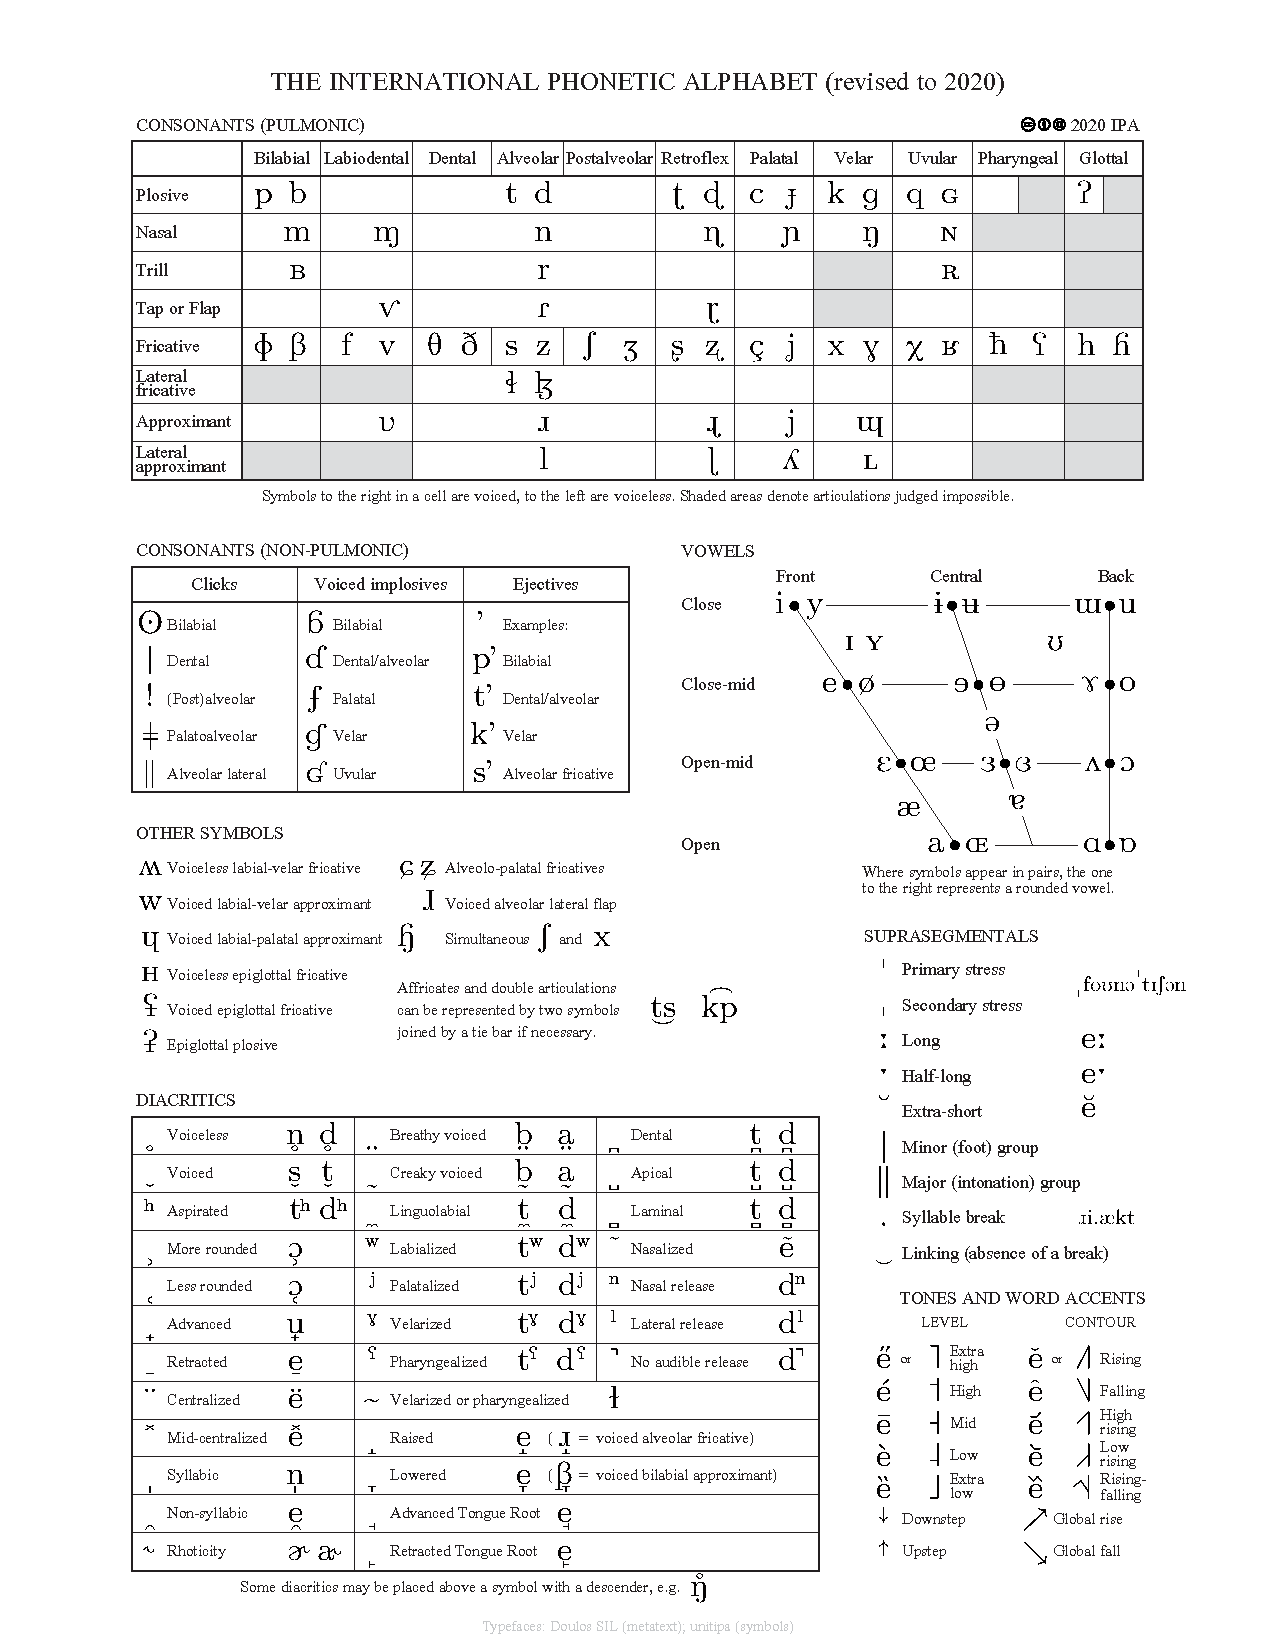
\includegraphics[width=0.9\textwidth]{figures/IPA_unitipa_2020_full.pdf}
    \caption{\href{http://www.internationalphoneticassociation.org/content/ipa-chart}{IPA Chart}, available under a Creative Commons Attribution-Sharealike 3.0 Unported License. 
    Copyright © 2018 International Phonetic Association.}
    \label{fig:ipa_chart}
\end{figure}

\section{Extended Results}
\begin{table}[ht]
    \centering
    \resizebox{\textwidth}{!}{%
    \input{pages/results_table.tex} 
    }
    \caption{Summary of the Results}
    \label{tab:results-summary}
\end{table}

\begin{figure}[H]  
    \centering
    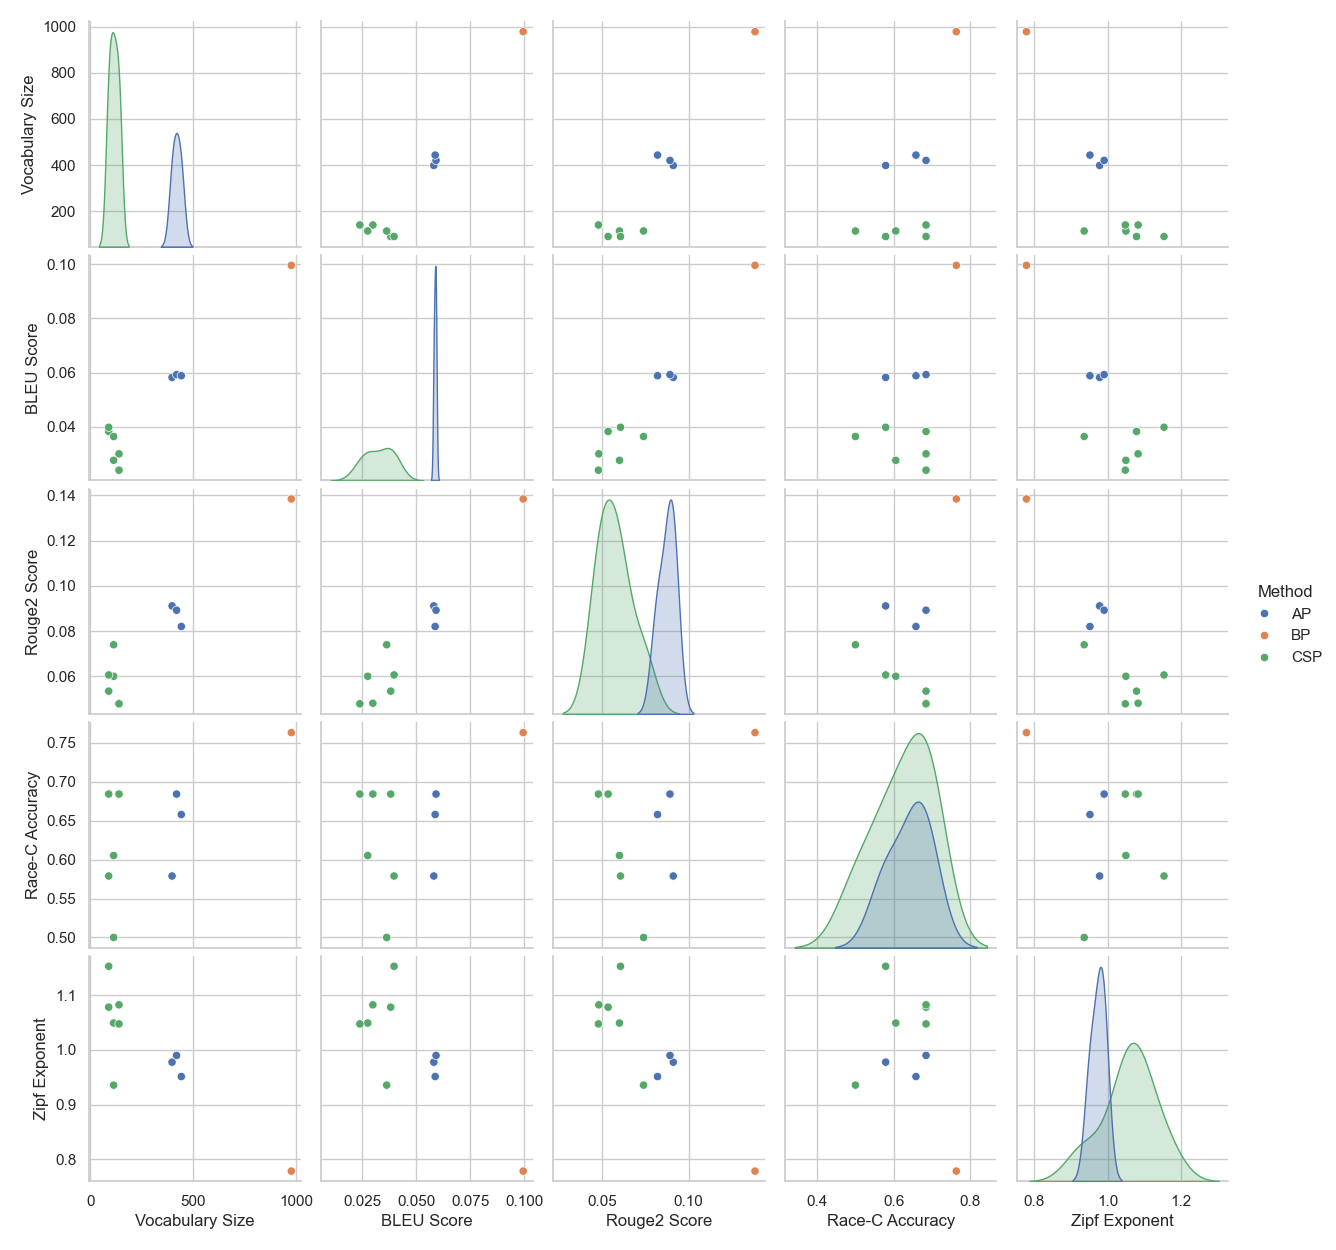
\includegraphics[width=0.9\linewidth]{figures/results/0_pairplot_vocabulary.png}
    \caption{Comparing different Simplifying vocabulary generation methods with the baseline.}
    \label{fig:compare-vocab-gen-types}
\end{figure}

\section{Sample Language generated from Baseline Pipeline}

\begin{longtable}{|l|p{10cm}|}
\hline
\textbf{Feature} & \textbf{Implementation} \\
\hline
\endhead

Language Name & \textipa{wi:di} \\
\hline
Standard Word Order & The language has the following standard word order: SOV \\
\hline
Agglutinative & The language is primarily agglutinative, i.e., complex words are formed by stringing together morphemes. \\
\hline
Noun & \begin{itemize}
  \item Cases:
    \begin{itemize}
      \item Nominative: unmarked
      \item Accusative: suffix `to`
      \item Dative: suffix `ti`
      \item Genitive: preposition `\textipa{fi:}`
      \item Instrumental: preposition `\textipa{Si}`
    \end{itemize}
  \item Number:
    \begin{itemize}
      \item Singular: unmarked
      \item Plural: prefix `\textipa{hu}`
    \end{itemize}
  \item Gender:
    \begin{itemize}
      \item Feminine: unmarked
      \item Masculine: suffix `\textipa{Ja}`
      \item Neuter: suffix `\textipa{te}`
    \end{itemize}
\end{itemize} \\
\hline
Article & \begin{itemize}
  \item Definite: particle after noun `\textipa{tE}`
  \item Indefinite: particle after noun `\textipa{nu}`
\end{itemize} \\
\hline
Demonstrative & \begin{itemize}
  \item Proximal (this): `\textipa{fE}`
  \item Distal (that): `\textipa{tSi:}`
\end{itemize} \\
\hline
Quantifier & \begin{itemize}
  \item Universal: `\textipa{Nga}`
  \item Small existential: `\textipa{ju}`
  \item Large existential: `\textipa{dZe}`
\end{itemize} \\
\hline
Adjective & \begin{itemize}
  \item Positive: unmarked
  \item Comparative: suffix `\textipa{dZi:}`
  \item Superlative: prefix `\textipa{Ja}`
\end{itemize} \\
\hline
Adverb & \begin{itemize}
  \item Positive: unmarked
  \item Comparative: suffix `\textipa{de}`
  \item Superlative: prefix `\textipa{te}`
\end{itemize} \\
\hline
Pronoun & \begin{itemize}
  \item 1st: `\textipa{io}`, 2nd: `\textipa{tu}`, 3rd: `\textipa{lei}`
  \item Cases: nominative (unmarked), accusative `\textipa{Je}`, dative `\textipa{tSa}`, genitive `\textipa{me}`, instrumental `\textipa{mO}`
  \item Gender: masculine `\textipa{tSu}`, neuter `\textipa{tE}`, feminine unmarked
\end{itemize} \\
\hline
Tense & \begin{itemize}
  \item Present: unmarked
  \item Past: prefix `\textipa{mo}`
  \item Future: prefix `\textipa{fo}`
\end{itemize} \\
\hline
Aspect & \begin{itemize}
  \item Perfective: unmarked
  \item Imperfective: suffix `\textipa{rO}`
\end{itemize} \\
\hline
Mood & Grammatical mood indicated by auxiliary verbs \\
\hline
Coordination & \begin{itemize}
  \item and: A `\textipa{Ni:}` B
  \item or: A `\textipa{SO}` B
  \item but: A `\textipa{gE}` B
  \item so: A `\textipa{dZa}` B
\end{itemize} \\
\hline
Subordination & \begin{itemize}
  \item because: A `\textipa{le}` B
  \item if: A `\textipa{zo}` B
  \item before: A `\textipa{hi:}` B
\end{itemize} \\
\hline
Verb Negation & Negation with the particle `\textipa{re}` before the verb \\
\hline
Question Formation & Word order changes to SVO with a `?`. Wh-words:
\begin{itemize}
  \item Who/What: `\textipa{sa}`
  \item When: `\textipa{tSi}`
  \item Where: `\textipa{NO}`
  \item Why: `\textipa{fO}`
  \item How: `\textipa{rO}`
  \item How Much/Many: `\textipa{ro}`
\end{itemize} \\
\hline
Yes/No Answers & Answered by echoing the verb, with or without negation \\
\hline
\end{longtable}

\begin{figure}[H]
    \centering
    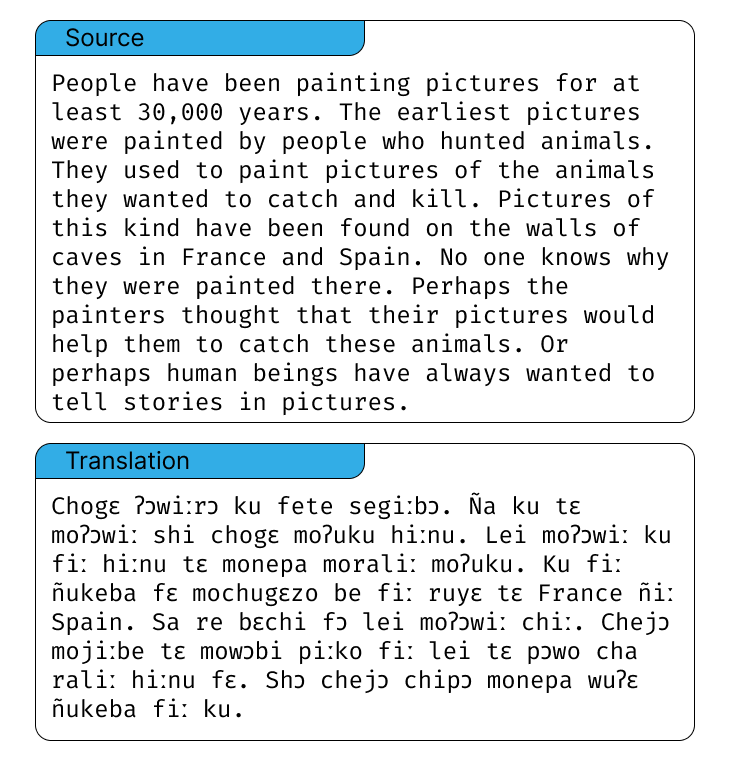
\includegraphics[width=0.9\linewidth]{figures/bp_22_8_source_trans.png}
    \caption{Source and Translation sample from the Baseline pipeline.}
    \label{fig:source_trans-bp}
\end{figure}

\section{Sample Language generated from Approximating Pipeline with 23 phonemes}

\begin{longtable}{|l|p{10cm}|}
\hline
\textbf{Feature} & \textbf{Implementation} \\
\hline
\endhead

Language Name & mangochote \\
\hline

StandardWordOrder & The language has the following standard word order: SOV \\
\hline

Agglutinative & The language is primarily agglutinative, i.e. complex words are formed by stringing together morphemes. \\
\hline

Noun & All nouns have the following features:
\begin{itemize}
    \item The language implements the following cases with the corresponding markers:
    \begin{itemize}
        \item The nominative case is not marked.
        \item The accusative case is marked by the suffix: 'ha'
        \item The dative case is marked by the suffix: 'no'
        \item The genitive case is marked by the preposition: 'wi'
        \item The instrumental case is marked by the preposition: 'ta'
    \end{itemize}
    \item Number:
    \begin{itemize}
        \item Singular is not marked.
        \item Plural is marked by the prefix: 're'
    \end{itemize}
    \item The language implements the following genders with the corresponding markers:
    \begin{itemize}
        \item Feminine is not marked.
        \item Masculine is marked by the suffix: 'tu'
        \item Neuter is marked by the suffix: 'nu'
    \end{itemize}
\end{itemize} \\
\hline

Article & Articles have the following features:
\begin{itemize}
    \item Definite (the) article is expressed using particle after the noun: 'yu'
    \item Indefinite (a) article is expressed using particle after the noun: 'ke'
\end{itemize} \\
\hline

Demonstrative & Demonstratives have the following features:
\begin{itemize}
    \item Proximal (this) is expressed using particle: 'po'
    \item Distal (that) is expressed using particle: 'ri'
\end{itemize} \\
\hline

Quantifier & Quantifiers have the following features:
\begin{itemize}
    \item Universal (all, every, each, both) is expressed using particle: 'bu'
    \item Small existential (some, a few) is expressed using particle: 'gu'
    \item Large existential (many, several) is expressed using particle: 're'
\end{itemize} \\
\hline

Adjective & All adjectives have the following features:
\begin{itemize}
    \item The language implements the following grammatical degrees with the corresponding markers:
    \begin{itemize}
        \item Positive degree is not marked.
        \item Comparative is marked by the suffix: 'ya'
        \item Superlative is marked by the prefix: 'tu'
    \end{itemize}
\end{itemize} \\
\hline

Adverb & The adverbs of this language have the following features:
\begin{itemize}
    \item The language implements the following grammatical degrees with the corresponding markers:
    \begin{itemize}
        \item Positive degree is not marked.
        \item Comparative is marked by the suffix: 'ro'
        \item Superlative is marked by the prefix: 'nu'
    \end{itemize}
\end{itemize} \\
\hline

Pronoun & Pronouns have the following features:
\begin{itemize}
    \item Persons:
    \begin{itemize}
        \item First person: 'io'
        \item Second person: 'tu'
        \item Third person: 'lei'
    \end{itemize}
    \item The language implements the following cases with the corresponding markers:
    \begin{itemize}
        \item The nominative case is not marked.
        \item The accusative case is marked by the suffix: 'gi'
        \item The dative case is marked by the suffix: 'ta'
        \item The genitive case is marked by the preposition: 'pa'
        \item The instrumental case is marked by the preposition: 'pi'
    \end{itemize}
    \item The language implements the following genders with the corresponding markers:
    \begin{itemize}
        \item Feminine is not marked.
        \item Masculine is marked by the suffix: 'ga'
        \item Neuter is marked by the suffix: 'cha'
    \end{itemize}
\end{itemize} \\
\hline

Tense & The language uses the following tenses:
\begin{itemize}
    \item Verbs in the present tense are not marked by any markers.
    \item Verbs in the past tense are marked by the prefix 'li'.
    \item Verbs in the future tense are marked by the prefix 'pe'.
\end{itemize} \\
\hline

Aspect & The language uses the following aspects:
\begin{itemize}
    \item Verbs in the perfective aspect are not marked by any markers.
    \item Verbs in the imperfective aspect are marked by the suffix 're'.
\end{itemize} \\
\hline

Mood & Grammatical Mood is indicated by auxiliary verbs \\
\hline

Coordination & Two Clauses A and B can be coordinated using the following particles:
\begin{itemize}
    \item cumulative (and): A da B
    \item alternative (or): A do B
    \item adversative (but): A che B
    \item illative (therefore, so): A na B
\end{itemize} \\
\hline

Subordination & Two Clauses A and B can be subordinated using the following particles:
\begin{itemize}
    \item causal (because): A yi B
    \item conditional (if): A nga B
    \item preceding\_temporal (before): A ko B
\end{itemize} \\
\hline

Verb Negation & The language uses the particle 'yo' before the verb to negate it. \\
\hline

Question Formation & The language forms questions by:
\begin{itemize}
    \item Changing the word order to SVO
    \item Adding a '?' at the end of the question
    \item The language uses the following words for W questions:
    \begin{itemize}
        \item Who, What: ba
        \item When: ro
        \item Where: lu
        \item Why: la
        \item How: gi
        \item How Much, How Many: wu
    \end{itemize}
\end{itemize} \\
\hline

Yes/No Answers & There are no separate Yes or No words. Yes/No questions can be answered by echoing the verb in the question with or without negation. \\
\hline

\end{longtable}

\begin{figure}[H]
	\centering
	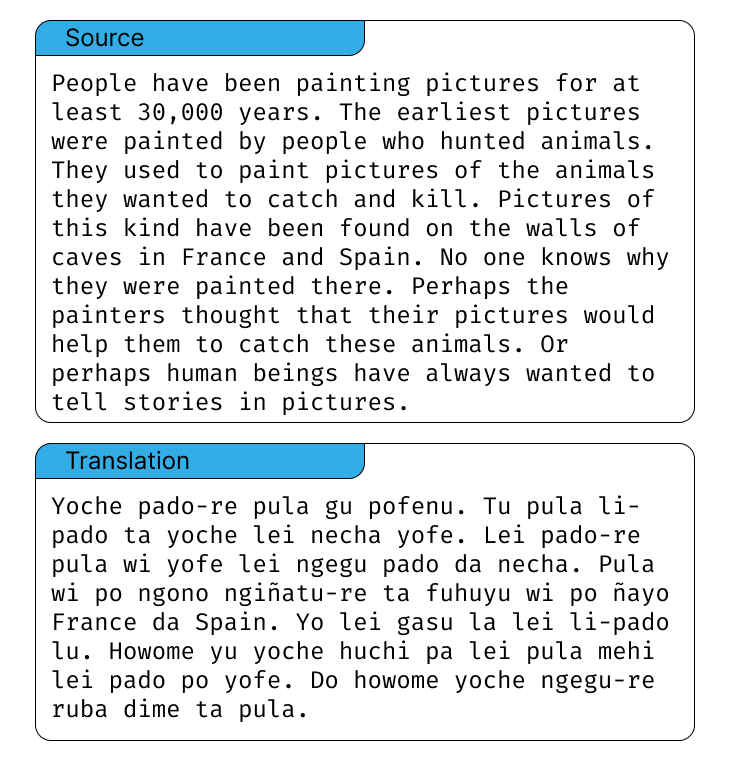
\includegraphics[width=0.9\linewidth]{figures/ap_18_5_source_trans.png}
	\caption{Source and Translation sample from the Approximating pipeline with 23 phonemes.}
	\label{fig:source_trans-ap}
\end{figure}